\chapter{Probability for Data Analysis}
\label{ch:probability-data-analysis}

Data describe what has been observed. Probability describes uncertainty about
what may be observed next and provides the language needed to connect a sample
to a wider process. In engineering, that uncertainty may concern a component
failure, a packet loss, a false alarm, or the unknown cause of a detected
fault.

This chapter follows the notation and core definitions in \emph{Mathematics
for Software Engineering}, but selects only the material needed for practical
data analysis. We use events, tables, and probability trees rather than a
catalogue of counting formulas. The binomial coefficient is introduced in
Chapter~\ref{ch:discrete-distributions}, where it is needed.

\section{Engineering question and learning outcomes}

Our running example is an automated optical inspection system that flags
possible solder defects on circuit boards. We ask:

\begin{quote}
When the inspection system flags a board, how strongly should that result
change our belief that the board is actually defective?
\end{quote}

After studying this chapter, you should be able to:
\begin{itemize}
    \item represent a random experiment using a sample space and events;
    \item translate not, and, and or into complements, intersections, and unions;
    \item use complement and addition rules without double-counting;
    \item calculate conditional probabilities from a contingency table;
    \item distinguish mutually exclusive events from independent events;
    \item use multiplication rules and probability trees;
    \item apply the law of total probability and Bayes' theorem; and
    \item distinguish sensitivity, false-positive rate, and positive
          predictive value.
\end{itemize}

\section{Random experiments, sample spaces, and events}

\begin{definition}[Random experiment]
A \textbf{random experiment} is a repeatable process whose outcome is not
known with certainty before it is observed.
\end{definition}

Random does not mean unstructured. Repeated trials under apparently similar
conditions can produce different outcomes, and this uncertainty is part of
the model.

\begin{definition}[Sample space, outcome, and event]
The \textbf{sample space}, denoted by $S$, is the set of all possible outcomes
of a random experiment. An \textbf{outcome} is one element of $S$. An
\textbf{event} is a subset of $S$.
\end{definition}

The sample space depends on the question. For one board, it could be
\[
    S=\{\text{flagged},\text{not flagged}\}.
\]
If the physical condition and test result are both relevant, use
\[
\begin{aligned}
S=\{&
(\text{defective},\text{flagged}),
(\text{defective},\text{not flagged}),\\
&
(\text{good},\text{flagged}),
(\text{good},\text{not flagged})\}.
\end{aligned}
\]
This representation makes false positives and false negatives visible.

Let $D$ denote a defective board and $F$ a flag:
\begin{itemize}
    \item $D^c$: the board is not defective;
    \item $D\cap F$: the board is defective and flagged;
    \item $D\cup F$: the board is defective or flagged, including both; and
    \item $D-F=D\cap F^c$: the board is defective but not flagged.
\end{itemize}
In probability, or is inclusive unless but not both is stated.

\subsection*{Probability as a model}

A probability may come from a physical model, long-run relative frequencies,
historical data, or explicit engineering judgement. Whatever its origin, it
must satisfy the following rules.

\begin{definition}[Probability rules]
A probability model satisfies:
\begin{enumerate}
    \item $0\leq P(A)\leq 1$ for every event $A$;
    \item $P(S)=1$; and
    \item if $A_1,A_2,\ldots$ are mutually exclusive, then
    \[
        P\left(\bigcup_i A_i\right)=\sum_i P(A_i).
    \]
\end{enumerate}
\end{definition}

An empirical failure rate is not automatically a timeless law. A rate
estimated under one operating condition may be inappropriate after a process
change.

\section{Complements, unions, and intersections}

\begin{theorem}[Complement and addition rules]
For events $A$ and $B$,
\[
    P(A^c)=1-P(A)
\]
and
\[
    P(A\cup B)=P(A)+P(B)-P(A\cap B).
\]
If $A$ and $B$ are mutually exclusive, $P(A\cap B)=0$.
\end{theorem}

The subtraction prevents the intersection from being counted twice.

\begin{example}[Two inspection warnings]
Suppose 12\% of boards trigger a solder warning, 7\% trigger an alignment
warning, and 3\% trigger both. If $S_o$ and $A_l$ denote the events, then
\[
P(S_o\cup A_l)=0.12+0.07-0.03=0.16.
\]
Thus, 16\% trigger at least one warning.
\end{example}

The complement rule is often easiest for at least one. If three independent
backup components each fail with probability 0.02, the probability that at
least one fails is
\[
    1-(1-0.02)^3\approx 0.0588.
\]
The multiplication requires independence.

\section{Conditional probability and contingency tables}

New information changes the reference group. If a board is known to be
flagged, compare it only with flagged boards.

\begin{definition}[Conditional probability]
For events $A$ and $B$ with $P(B)>0$,
\[
    P(A\mid B)=\frac{P(A\cap B)}{P(B)}.
\]
\end{definition}

The condition is to the right of the vertical bar. In general,
\[
    P(F\mid D)\neq P(D\mid F).
\]
The first asks how the test behaves among defective boards; the second asks
how many flagged boards are actually defective.

\subsection*{Natural frequencies}

Suppose historical information gives
\[
P(D)=0.02,\qquad P(F\mid D)=0.95,\qquad
P(F\mid D^c)=0.08.
\]
For a hypothetical batch of 10,000 boards, the expected counts are:

\begin{table}[htbp]
\centering
\renewcommand{\arraystretch}{1.25}
\begin{tabular}{lrrr}
\toprule
& \textbf{Flagged} & \textbf{Not flagged} & \textbf{Total}\\
\midrule
Defective & 190 & 10 & 200\\
Good & 784 & 9016 & 9800\\
\midrule
Total & 974 & 9026 & 10000\\
\bottomrule
\end{tabular}
\caption{Natural-frequency representation of the inspection model. Counts
are expected counts, not newly observed data.}
\label{tab:ch2-confusion}
\end{table}

The table gives
\[
\begin{aligned}
P(F\mid D)&=\frac{190}{200}=0.95,\\
P(F\mid D^c)&=\frac{784}{9800}=0.08,\\
P(D\mid F)&=\frac{190}{974}\approx 0.195.
\end{aligned}
\]
These are sensitivity, false-positive rate, and positive predictive value,
respectively. A sensitivity of 95\% does not imply that 95\% of flagged
boards are defective.

\section{Multiplication rules and probability trees}

\begin{theorem}[Multiplication rule]
For events $A$ and $B$,
\[
    P(A\cap B)=P(A)P(B\mid A)=P(B)P(A\mid B),
\]
whenever the stated conditional probabilities are defined.
\end{theorem}

A probability tree starts with a base-rate branch and continues with
conditional branches. Multiply along a path and add mutually exclusive paths.

\begin{figure}[htbp]
\centering
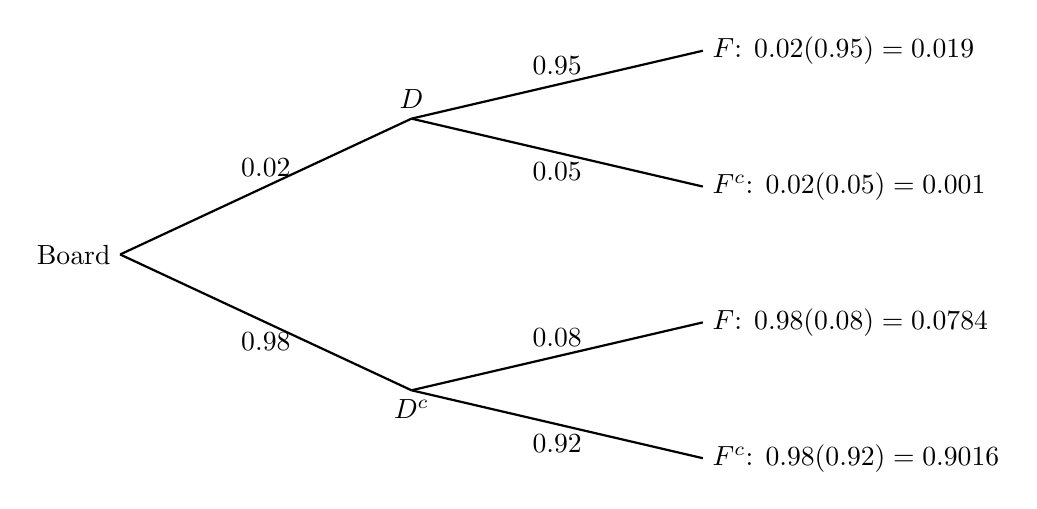
\begin{tikzpicture}[x=3.7cm,y=1.15cm]
  \coordinate (root) at (0,0);
  \coordinate (d) at (1,1.5);
  \coordinate (g) at (1,-1.5);
  \coordinate (df) at (2,2.25);
  \coordinate (dn) at (2,0.75);
  \coordinate (gf) at (2,-0.75);
  \coordinate (gn) at (2,-2.25);
  \draw[thick] (root) -- node[above] {$0.02$} (d);
  \draw[thick] (root) -- node[below] {$0.98$} (g);
  \draw[thick] (d) -- node[above] {$0.95$} (df);
  \draw[thick] (d) -- node[below] {$0.05$} (dn);
  \draw[thick] (g) -- node[above] {$0.08$} (gf);
  \draw[thick] (g) -- node[below] {$0.92$} (gn);
  \node[left] at (root) {Board};
  \node[above] at (d) {$D$};
  \node[below] at (g) {$D^c$};
  \node[right] at (df) {$F$: $0.02(0.95)=0.019$};
  \node[right] at (dn) {$F^c$: $0.02(0.05)=0.001$};
  \node[right] at (gf) {$F$: $0.98(0.08)=0.0784$};
  \node[right] at (gn) {$F^c$: $0.98(0.92)=0.9016$};
\end{tikzpicture}
\caption{Probability tree for the optical inspection system.}
\label{fig:ch2-tree}
\end{figure}

\section{Independence and mutual exclusivity}

\begin{definition}[Independence]
Events $A$ and $B$ are \textbf{independent} if
\[
    P(A\cap B)=P(A)P(B).
\]
When $P(B)>0$, this is equivalent to $P(A\mid B)=P(A)$.
\end{definition}

Independence means that learning whether one event occurred does not change
the probability of the other. It must be supported by the process or model,
not assumed for convenience.

\begin{definition}[Mutually exclusive events]
Events $A$ and $B$ are \textbf{mutually exclusive} if
$A\cap B=\emptyset$.
\end{definition}

If mutually exclusive events both have positive probability, observing one
rules out the other, so they are dependent. For example, $F$ and $F^c$ are
mutually exclusive but not independent when $0<P(F)<1$. Results from
consecutive boards should be modelled as independent only if common machine
drift or batch effects are negligible.

\section{Total probability and Bayes' theorem}

A set of mutually exclusive events whose union is $S$ is a
\textbf{partition}. Events $D$ and $D^c$ partition the board population.

\begin{theorem}[Law of total probability]
If $B_1,\ldots,B_k$ form a partition of $S$, then
\[
    P(A)=\sum_{i=1}^{k}P(A\mid B_i)P(B_i).
\]
\end{theorem}

For the inspection system,
\[
\begin{aligned}
P(F)&=P(F\mid D)P(D)+P(F\mid D^c)P(D^c)\\
&=0.95(0.02)+0.08(0.98)=0.0974.
\end{aligned}
\]

\begin{theorem}[Bayes' theorem]
If $B_1,\ldots,B_k$ form a partition and $P(A)>0$, then
\[
P(B_j\mid A)=
\frac{P(A\mid B_j)P(B_j)}
{\sum_{i=1}^{k}P(A\mid B_i)P(B_i)}.
\]
For a two-part partition,
\[
P(B\mid A)=
\frac{P(A\mid B)P(B)}
{P(A\mid B)P(B)+P(A\mid B^c)P(B^c)}.
\]
\end{theorem}

Bayes' theorem reverses the direction of conditioning. The numerator is the
joint probability of the hypothesis and evidence; the denominator is the
total probability of the evidence across every path.

\section{Worked engineering example}

\[
\begin{aligned}
P(D\mid F)
&=\frac{P(F\mid D)P(D)}
{P(F\mid D)P(D)+P(F\mid D^c)P(D^c)}\\
&=\frac{0.95(0.02)}{0.95(0.02)+0.08(0.98)}
\approx 0.195.
\end{aligned}
\]

A flagged board has a 19.5\% probability of being defective under this model.
About 80.5\% of flags are false positives. This does not contradict the 95\%
sensitivity: 190 of 200 defective boards are caught, but the much larger
group of good boards produces 784 false alarms.

A flag still increases risk from the 2\% base rate to 19.5\%. Whether that is
sufficient to scrap a board depends on the costs of confirmation, missed
defects, and unnecessary scrap. A sensible workflow may send flagged boards
to a more accurate confirmatory test.

The same inspection system produces different predictive values in
populations with different defect rates.

\clearpage
\section{Python in practice}

Figure~\ref{fig:ch2-base-rate} visualises the base-rate effect before we
reproduce the calculation in Python.

\begin{figure}[htbp]
    \centering
    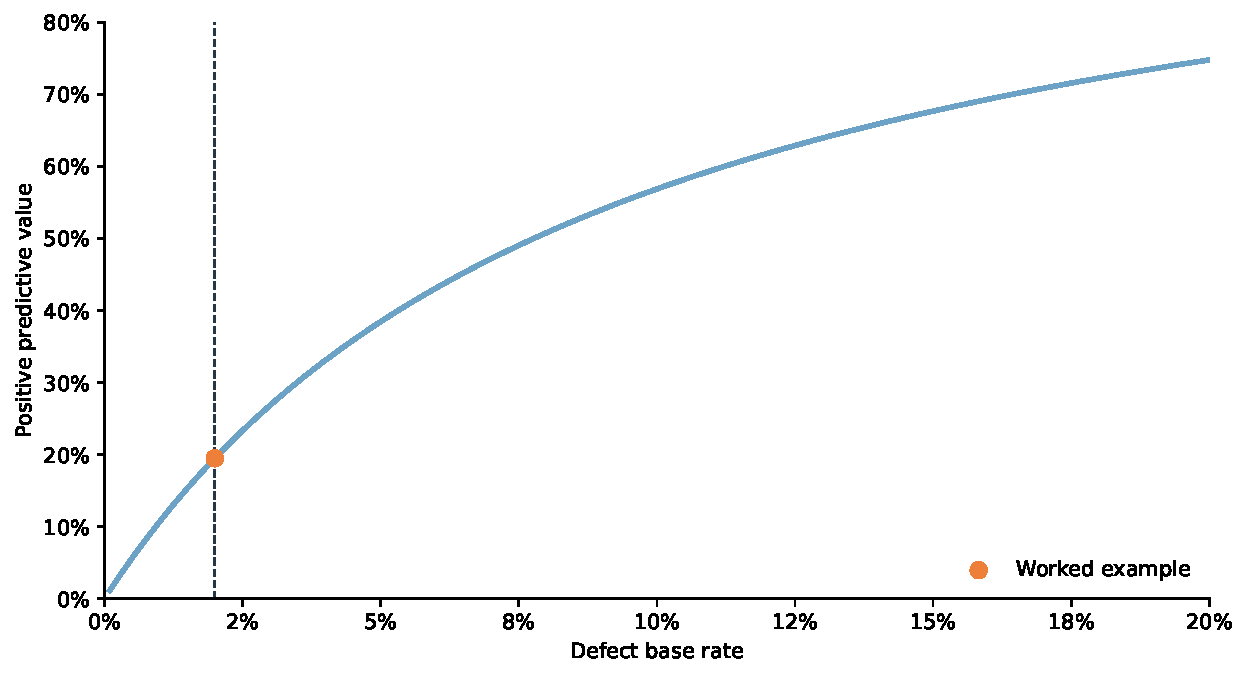
\includegraphics[width=0.88\textwidth]{figure/chapter02_base_rate.pdf}
    \caption{Positive predictive value as a function of defect base rate for
    sensitivity 0.95 and false-positive rate 0.08.}
    \label{fig:ch2-base-rate}
\end{figure}

\begin{python}
import numpy as np
import pandas as pd
import matplotlib.pyplot as plt

p_defect = 0.02
sensitivity = 0.95
false_positive_rate = 0.08

p_flag = (
    sensitivity * p_defect
    + false_positive_rate * (1 - p_defect)
)
ppv = sensitivity * p_defect / p_flag

print(f"P(flag) = {p_flag:.4f}")
print(f"P(defect | flag) = {ppv:.4f}")
\end{python}

Natural frequencies make the denominators visible:

\begin{python}
n = 10_000
n_defective = round(n * p_defect)
n_good = n - n_defective

tp = round(n_defective * sensitivity)
fn = n_defective - tp
fp = round(n_good * false_positive_rate)
tn = n_good - fp

table = pd.DataFrame(
    {"flagged": [tp, fp], "not_flagged": [fn, tn]},
    index=["defective", "good"],
)
table["total"] = table.sum(axis=1)
table.loc["total"] = table.sum(axis=0)
print(table)
\end{python}

Simulation checks the long-run interpretation, but does not replace the exact
calculation:

\begin{python}
rng = np.random.default_rng(2026)
n_sim = 100_000

defective = rng.random(n_sim) < p_defect
flagged = np.where(
    defective,
    rng.random(n_sim) < sensitivity,
    rng.random(n_sim) < false_positive_rate,
)

simulated_ppv = defective[flagged].mean()
print(f"Simulated P(defect | flag) = {simulated_ppv:.4f}")
\end{python}

\begin{quote}
Under a 2\% defect base rate, 95\% sensitivity, and an 8\% false-positive
rate, a flagged board has a 19.5\% probability of being defective. A flag
should trigger confirmation rather than be treated as proof.
\end{quote}

\section{Common pitfalls and chapter summary}

\subsection*{Common pitfalls}
\begin{itemize}
    \item \textbf{Reversing the condition.} $P(F\mid D)$ and $P(D\mid F)$ answer
          different questions.
    \item \textbf{Ignoring the base rate.} Sensitivity alone cannot determine
          positive predictive value.
    \item \textbf{Double-counting a union.} Subtract $P(A\cap B)$ unless the
          events are mutually exclusive.
    \item \textbf{Confusing exclusivity with independence.} Disjoint
          positive-probability events are dependent.
    \item \textbf{Multiplying marginal probabilities automatically.}
          $P(A\cap B)=P(A)P(B)$ requires independence.
    \item \textbf{Treating inputs as timeless facts.} Base rates and error
          rates can change across populations and conditions.
\end{itemize}

\subsection*{Chapter summary}

Events are subsets of a sample space. Complements handle not, intersections
handle and, and unions handle inclusive or. Conditional probability changes
the reference group. Independence means conditioning does not change a
probability; it is not mutual exclusivity. Probability trees and the
multiplication rule construct joint probabilities, total probability adds
mutually exclusive paths, and Bayes' theorem reverses conditioning.

\clearpage
\section{Exercises}

\begin{enumerate}
    \item A server request can succeed, time out, or return an application
    error. Define a sample space and the event that the request fails. Explain
    how the sample space changes if response time is recorded continuously.

    \item Let $P(A)=0.18$, $P(B)=0.25$, and $P(A\cap B)=0.09$ for memory and
    latency warnings. Find $P(A\cup B)$, $P(A-B)$, and the probability of
    neither warning.

    \item A quality sample contains 72 flagged defective items, 8 unflagged
    defective items, 45 flagged good items, and 875 unflagged good items.
    Compute sensitivity, false-positive rate, positive predictive value,
    negative predictive value, and accuracy. Interpret each denominator.

    \item Give one engineering example of mutually exclusive events and one
    of events that could reasonably be independent. Justify both.

    \item A component comes from line A with probability 0.65 and line B with
    probability 0.35. Failure probabilities are 0.01 and 0.04. Draw a tree,
    find the overall failure probability, and find the probability that a
    failed component came from line B.

    \item Reproduce Table~\ref{tab:ch2-confusion} in Pandas and verify the
    three displayed conditional probabilities from its row and column totals.

    \item Reproduce Figure~\ref{fig:ch2-base-rate}. Compare predictive value
    at base rates 0.5\%, 2\%, 10\%, and 20\%. Explain why sensitivity alone is
    insufficient.

    \item Simulate the inspection example for $n=1000$, $10\,000$, and
    $100\,000$ with \texttt{default\_rng(2026)}. Compare with the exact result.

    \item Reduce the false-positive rate from 0.08 to 0.01 while sensitivity
    remains 0.95. Calculate the new predictive value and expected false alarms
    per 10,000 boards.

    \item Correct the claim that a detector with 95\% sensitivity gives every
    flagged board a 95\% probability of being defective.
\end{enumerate}
